\begin{center}
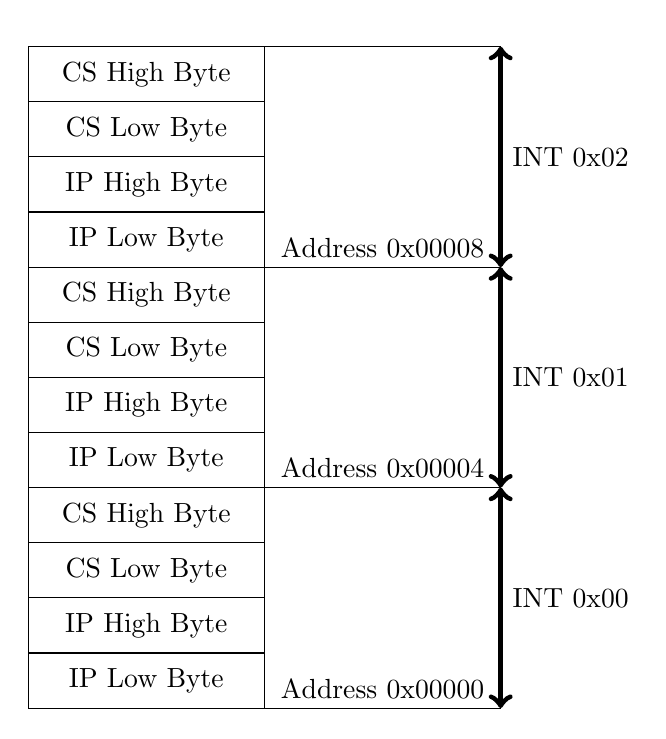
\begin{tikzpicture}
\label{figRootKitRealModeIVT}
\foreach \x in {0,2.8,5.6}
{
	\draw (0,\x) rectangle (3,\x+0.7) node [pos=0.5] {IP Low Byte};
	\draw (0,\x + 0.7) rectangle (3,\x+1.4) node [pos=0.5] {IP High Byte};	
	\draw (0,\x + 1.4) rectangle (3,\x+2.1) node [pos=0.5] {CS Low Byte};	
	\draw (0,\x + 2.1) rectangle (3,\x+2.8) node [pos=0.5] {CS High Byte};		
}
\draw (3,0) -- (6,0) node [pos = 0.5,above] {Address 0x00000};
\draw (3,2.8) -- (6,2.8) node [pos = 0.5,above] {Address 0x00004};
\draw (3,5.6) -- (6,5.6) node [pos = 0.5,above] {Address 0x00008};
\draw (3,8.4) -- (6,8.4) node [pos = 0.5,above] {};

\draw[<->, line width = 2pt] (6,0) -- (6,2.8) node [pos=0.5,right] {INT 0x00};
\draw[<->,line width = 2pt] (6,2.8) -- (6,5.6) node [pos=0.5,right] {INT 0x01};
\draw[<->,line width = 2pt] (6,5.6) -- (6,8.4) node [pos=0.5,right] {INT 0x02};
\end{tikzpicture}
\end{center}